\documentclass[12pt, a4paper]{article}
\usepackage[utf8]{inputenc}
\usepackage[spanish]{babel}
\usepackage{hyperref}

\usepackage{pdfpages} %para insertar pdfs

\setlength{\parindent}{0em}
\setlength{\parskip}{1em}

\usepackage{graphicx} %package to manage images
\usepackage{float}% If comment this, figure moves to Page 2
\graphicspath{ {images/} }

%Title and authors
\title{%
    \begin{figure}[H]
        \centering
        
\includegraphics[width=0.7\textwidth]{Logo_EHU.png}
    \end{figure}
  \textbf{Ingeniería del Software} \\
  \large{Sprint 1 Sunken \\
            2021-2022\\
            ...\\
            \textbf{Titulación:}\\
            Grado en Informática de Gestión y Sistemas de Información\\
            ...\\
            2º Curso(2º Cuatrimestre)
    }
}\usepackage{graphicx} %package to manage images
\usepackage{float}% If comment this, figure moves to Page 2
\graphicspath{ {images/} }

\author{Alan García, Álvaro Díez-Andino, \\Danel Alonso, Gorka Crespo, Adrián López}

\begin{document}
\maketitle
\newpage
\tableofcontents
\newpage

% ---------- INFORME MVC ----------
\section{Informe MVC}
El MVC es el protocolo que se encarga de los observers y los observables que utilizamos para actualizar los visuales de nuestro juego.

En el aspecto gráfico, se crea una ventana principal que se encargará de visualizar el estado actual de la aplicación. La vista se comunica con el modelo (el juego) a través del controlador (\textit{ControladorVentanaPrincipal}) que se encarga de gestionar todas las acciones relacionadas con el mouse y el selector de orientación ya que implementa MouseListener e ItemListener. Además, en la vista se crean dos tableros de 10x10 cada uno, el panel de barcos donde estarán los botones para seleccionar el tipo de barco, el panel de misiles (de momento solo bomba) y además el seleccionador de dirección para colocar los barcos (Norte,Sur,Este,Oeste).

Al pasar por encima de alguna casilla con el cursor, estas cambiarán de color mientras el cursor se encuentre en su area. El controlador gestiona la posición del mouse y le indica a la casilla correspondiente que cambie su color al color del hover.

Cuando se selecciona un barco, misil, orientación… Se actualiza el registro del controlador con la información que se ha seleccionado para posteriormente enviarla a Gestor del Juego un formulario con todos los datos necesarios. 

Al hacer 'click' en una casilla se produce la llamada al Gestor del Juego y se envía el formulario previamente mencionado:\textit{notificarCasillaPresionada()}.

Una vez el Gestor del Juego ha realizado los cambios en el estado de la aplicación se actualizan los estados de las casillas en la vista realizando una llamada a \textit{setChanged()} y \textit{notifyAll()} del patron Observer: el Gestor es el Observable y las casillas de la vista son los Observers.

% ---------- Actas de reunión ----------
\section{Actas de reunión}
Las actas de reunión están incluidas como un pdf adjunto.

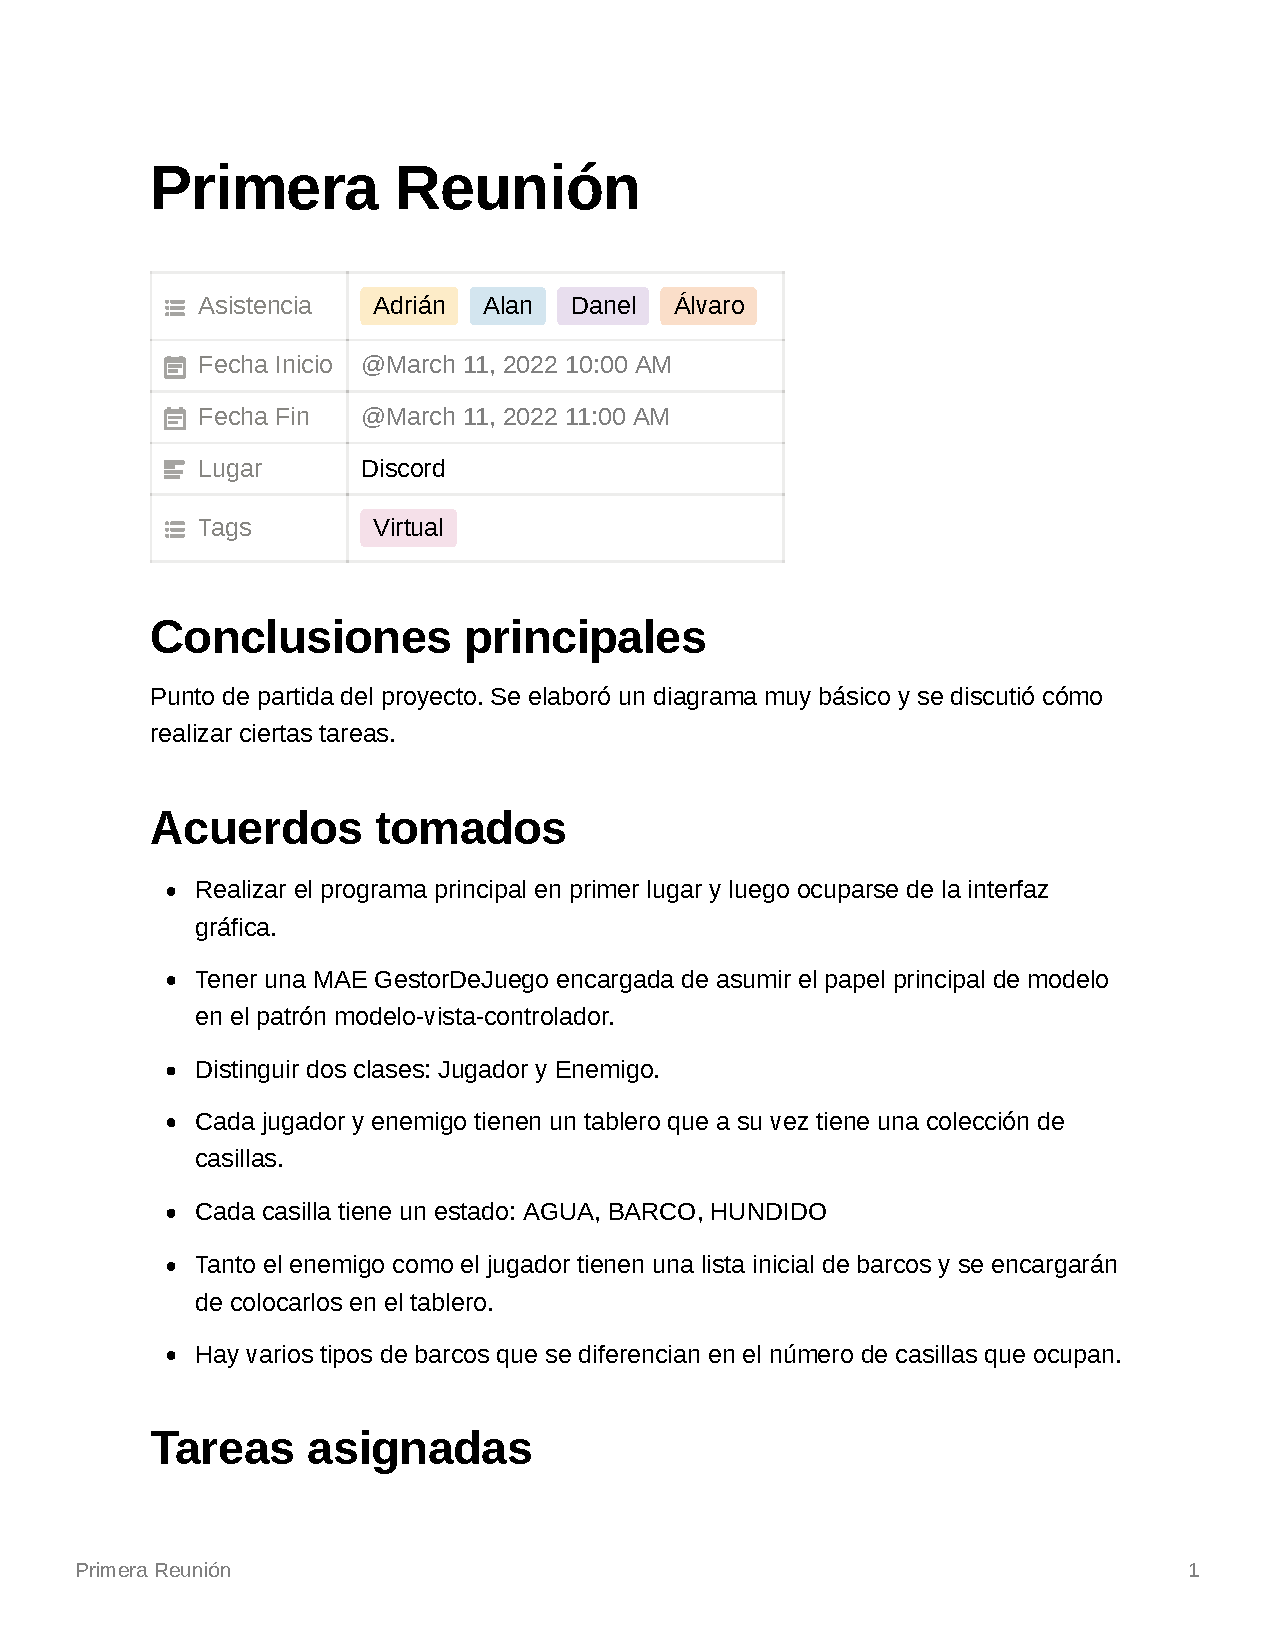
\includepdf[pages=-]{pdfs/actasReunion.pdf}
\end{document}